\documentclass{korigamik}

\usepackage{minted}
\usepackage{xcolor}
\usepackage{listings}
\usepackage{algpseudocode}
\usepackage[fleqn]{amsmath}
\usepackage{algorithm}
\usepackage{enumitem}

\title{Advanced Computer Networks}
\titlelabel{Lab Report}
\bottomnote{Department of Computer Science \& Engineering}
\author{Kushagra Lakhwani}
\rollno{2021UCI8036}
\semester{5th}
\course{CICPC16}
\logoimage{res/NSUT.png}{0.6}{Netaji Subhas University \\ of Technology}
\header{}

\colorlet{mycoolgray}{gray!40}
\lstdefinestyle{output}{
	numbers=none, % where to put the line-numbers
	numberstyle=\tiny, % the size of the fonts that are used for the line-numbers
	backgroundcolor=\color{darkgray},
	basicstyle=\ttfamily\color{white}\footnotesize,
	captionpos=b, % sets the caption-position to bottom
	breaklines=true, % sets automatic line breaking
	breakatwhitespace=false,
	keywordstyle=\color{white}\bfseries,
	language=bash,
}

\usepackage{tocloft}
\renewcommand{\cftsecafterpnum}{\qquad\rule{2cm}{0.4pt}}
\setcounter{tocdepth}{1}

\begin{document}

\maketitle
\newpage

\center\textbf{\large Abstract}

\begin{justify}
	The practical lab report \textit{``Operating Systems''} is the original and unmodified content submitted by \textit{Kushagra Lakhwani} (Roll No. 2021UCI8036).

	The report is submitted to \textit{Dr. Manoj Kumar} Department of Computer Science and Engineering, NSUT, Delhi, for the partial fulfillment of the requirements of the course \textit{``Operating Systems''} (CICPC09).
\end{justify}

\pagebreak


\thispagestyle{empty}
\tableofcontents
\newpage

\section{IPv4 Address Conversion}
\label{sec:ipv4}
\subsection{Objective}
To convert a binary IP address into dotted decimal and vice versa.
\subsection{Source Code}
\inputminted[firstline=5, lastline=39, fontsize=\footnotesize]{cpp}{code/ipv4.cpp}

\pagebreak

\subsection{Output}

\subsubsection{Binary to dotted decimal IP address}
\begin{lstlisting}[style=output]
$ ./ipv4
1. Binary to dotted decimal IP address
2. Dotted decimal to binary IP address
Enter your choice: 1
Enter binary IP address (32 bits): 11000000101010000000000100000001
Dotted Decimal IP address: 192.168.1.1
\end{lstlisting}

\subsubsection{Dotted decimal to binary IP address}

\begin{lstlisting}[style=output]
$ ./ipv4
1. Binary to dotted decimal IP address
2. Dotted decimal to binary IP address
Enter your choice: 2
Enter dotted decimal IP address (e.g., 192.168.1.1): 203.128.56.2
Binary IP address: 11001011100000000011100000000010
\end{lstlisting}

\pagebreak

\section{IP Address Classes}
\label{sec:ipclass}
\subsection{Objective}
To identify the class of an IP address.
\subsection{Theory}
In IPv4, IP addresses are divided into five classes: A, B, C, D, and E. Each
class has its own range of valid IP addresses and is used for specific
purposes.

\begin{enumerate}[label=\textbf{Class \Alph*:}, leftmargin=2cm]
	\item \begin{itemize}
		      \item Range: 1.0.0.0 to 126.255.255.255
		      \item Subnet Mask: 255.0.0.0
		      \item Address Allocation: Class A addresses are typically used by large organizations and corporations. They can support a very large number of hosts on a single network.
	      \end{itemize}
	      
	\item \begin{itemize}
		      \item Range: 128.0.0.0 to 191.255.255.255
		      \item Subnet Mask: 255.255.0.0
		      \item Address Allocation: Class B addresses are used by medium-sized organizations. They offer a moderate number of network and host addresses.
	      \end{itemize}
	      
	\item \begin{itemize}
		      \item Range: 192.0.0.0 to 223.255.255.255
		      \item Subnet Mask: 255.255.255.0
		      \item Address Allocation: Class C addresses are commonly used by small organizations and businesses. They provide a limited number of network addresses but a larger number of host addresses.
	      \end{itemize}
	      
	\item \begin{itemize}
		      \item Range: 224.0.0.0 to 239.255.255.255
		      \item Address Allocation: Class D addresses are reserved for multicast groups and are not used for traditional unicast communication. They are used for one-to-many or many-to-many communication.
	      \end{itemize}
	      
	\item \begin{itemize}
		      \item Range: 240.0.0.0 to 255.255.255.255
		      \item Address Allocation: Class E addresses are reserved for experimental or research purposes and are not typically used in public networks. They are reserved for future use and not intended for general use.
	      \end{itemize}
\end{enumerate}


\subsection{Source Code}

\inputminted[firstline=5, lastline=25, fontsize=\footnotesize]{cpp}{code/ipv4class.cpp}

\subsection{Output}

\begin{lstlisting}[style=output]
$ ./ipv4class
Enter an IPv4 address: 192.168.1.1
Class: C
\end{lstlisting}

\pagebreak


\section{Distance Vector Routing Algorithm}
\label{sec:Distance Vector Routing Algorithm}

\subsection{Objective}
To implement the Distance-Vector Routing algorithm.

\subsection{Theory}
A distance-vector routing (DVR) protocol requires that a router inform its
neighbors of topology changes periodically. Historically known as the old
\textbf{\textit{ARPANET}} routing algorithm or known as \textbf{\textit{Bellman-Ford}} algorithm.

Each router maintains a Distance Vector table containing the distance between
itself and \textit{all} possible destination nodes. Distances, based on a
chosen metric, are computed using information from the neighbors' distance
vectors.


\subsection{Information Kept by DV Router}
\begin{itemize}
	\item Each router has an ID.
	\item Associated with each link connected to a router, there is a link cost
	      (static or dynamic).
	\item Intermediate hops.
\end{itemize}

\subsection{Distance Vector Table Initialization}
\begin{itemize}
	\item Distance to itself = 0
	\item Distance to all other routers = infinity number.
\end{itemize}

\subsection{Distance Vector Algorithm}
\begin{enumerate}
	\item A router transmits its distance vector to each of its neighbors in a
	      routing packet.
	\item Each router receives and saves the most recently received distance
	      vector from each of its neighbors.
	\item A router recalculates its distance vector when:
	      \begin{itemize}
		      \item It receives a distance vector from a neighbor containing
		            different information than before.
		      \item It discovers that a link to a neighbor has gone down.
	      \end{itemize}
	\item The DV calculation is based on minimizing the cost to each destination:
	      \begin{align*}
		       & Dx(y) = \text{Estimate of least cost from x to y}               \\
		       & C(x,v) = \text{Node x knows cost to each neighbor v}            \\
		       & Dx = [Dx(y): y \in N] = \text{Node x maintains distance vector} \\
		       & \text{Node x also maintains its neighbors' distance vectors:}   \\
		       & \text{For each neighbor v, x maintains } Dv = [Dv(y): y \in N]
	      \end{align*}
\end{enumerate}

\pagebreak

\section{Bellman-Ford Algorithm}
\label{sec:Bellman-Ford Algorithm}

\subsection{Objective}
To implement the Bellman-Ford algorithm to find the shortest path
in a weighted graph.

\subsection{Theory}
The Bellman-Ford algorithm is used to find the shortest paths from a 
single source vertex to all other vertices in a weighted graph, even when the
graph contains negative weight edges. While it's not the most efficient
algorithm for all cases (especially for graphs with non-negative weights, where
Dijkstra's algorithm is typically faster),

\subsection{Source Code}
\inputminted[firstline=6, lastline=55, fontsize=\footnotesize]{cpp}{code/bellmanford.cpp}

\subsection{Output}
\begin{lstlisting}[style=output]
Enter the number of vertices and edges: 3 4
Enter edge 1 (source, destination, weight): 0 1 5
Enter edge 2 (source, destination, weight): 1 0 3
Enter edge 3 (source, destination, weight): 1 2 -1
Enter edge 4 (source, destination, weight): 2 0 1
Enter the source vertex: 2
Vertex  Distance from Source
0       1
1       6
2       0
\end{lstlisting}

\pagebreak

\section{Dijkstra's Algorithm}
\label{sec:Dijkstra's Algorithm}

\subsection{Objective}
To implement Dijkstra's algorithm to find the shortest path
in a weighted graph.

\subsection{Theory}
Dijkstra's algorithm is an algorithm for finding the shortest paths between
nodes in a graph, which may represent, for example, road networks. It was
conceived by computer scientist Edsger W. Dijkstra in 1956 and published three
years later.

Its time complexity is $O(|E| + |V| \log |V|)$, where $|E|$ is the number of
edges and $|V|$ is the number of vertices. However, this algorithm is only
applicable to graphs with positive edge weights.

\subsection{Source Code}

\inputminted[firstline=10, fontsize=\footnotesize]{cpp}{code/dijkstra.cpp}

\begin{figure}[ht]
	\centering
	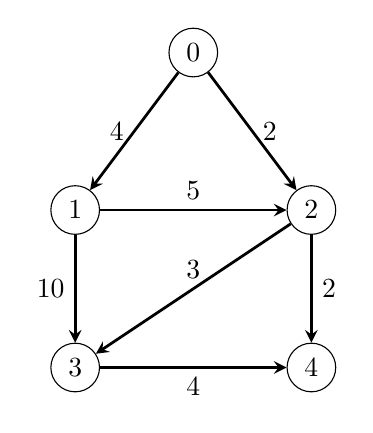
\begin{tikzpicture}[node distance=2.5cm, auto]
		\node[draw, circle] (0) at (4.5,2) {0};
		\node[draw, circle] (1) at (3,0) {1};
		\node[draw, circle] (2) at (6,0) {2};
		\node[draw, circle] (3) at (3,-2) {3};
		\node[draw, circle] (4) at (6,-2) {4};
		
		\draw[->, >=stealth, line width=1pt] (0) -- node[midway, left] {4} (1);
		\draw[->, >=stealth, line width=1pt] (0) -- node[midway, right] {2} (2);
		\draw[->, >=stealth, line width=1pt] (1) -- node[midway, above] {5} (2);
		\draw[->, >=stealth, line width=1pt] (1) -- node[midway, left] {10} (3);
		\draw[->, >=stealth, line width=1pt] (2) -- node[midway, above] {3} (3);
		\draw[->, >=stealth, line width=1pt] (2) -- node[midway, right] {2} (4);
		\draw[->, >=stealth, line width=1pt] (3) -- node[midway, below] {4} (4);
	\end{tikzpicture}
	\caption{Graph}
\end{figure}

\subsection{Output}

\begin{lstlisting}[style=output]
5 7
  0 1 4
  0 2 2
  1 2 5
  1 3 10
  2 3 3
  2 4 2
  3 4 4
0
Shortest distances from node 0:
Node 0: 0
Node 1: 4
Node 2: 2
Node 3: 5
Node 4: 4
\end{lstlisting}

\iffalse
	\begin{figure}[ht]
		\centering
		\begin{tikzpicture}
			% Nodes for locations
			\node[draw, circle] (A) at (0,0) {A};
			\node[draw, circle] (B) at (4,2) {B};
			\node[draw, circle] (C) at (6,0) {C};
			\node[draw, circle] (D) at (4,-3) {D};
			\node[draw, circle] (E) at (10,0) {E};
			
			% Routers
			\node[draw, rectangle] (RouterA) at (-1,-1) {Router A};
			\node[draw, rectangle] (RouterB) at (4,3) {Router B};
			\node[draw, rectangle] (RouterC) at (6,-1) {Router C};
			\node[draw, rectangle] (RouterD) at (5,-5) {Router D};
			\node[draw, rectangle] (RouterE) at (10,1) {Router E};
			
			% Computers
			\node[draw, circle] (CompA1) at (-3,-2) {Comp};
			\node[draw, circle] (CompA2) at (-3,-4) {Comp};
			\node[draw, circle] (CompB1) at (2,4) {Comp};
			\node[draw, circle] (CompB2) at (6,4) {Comp};
			\node[draw, circle] (CompC1) at (9,-2) {Comp};
			\node[draw, circle] (CompC2) at (8,-4) {Comp};
			\node[draw, circle] (CompD1) at (2,-6) {Comp};
			\node[draw, circle] (CompD2) at (6,-7) {Comp};
			\node[draw, circle] (CompE1) at (13,0) {Comp};
			\node[draw, circle] (CompE2) at (12,-2) {Comp};
			
			% Connections
			\draw[->] (A) -- (RouterA);
			\draw[->] (B) -- (RouterB);
			\draw[->] (C) -- (RouterC);
			\draw[->] (D) -- (RouterD);
			\draw[->] (E) -- (RouterE);
			
			% Connections between computers and routers
			\draw[->] (CompA1) -- (RouterA);
			\draw[->] (CompA2) -- (RouterA);
			\draw[->] (CompB1) -- (RouterB);
			\draw[->] (CompB2) -- (RouterB);
			\draw[->] (CompC1) -- (RouterC);
			\draw[->] (CompC2) -- (RouterC);
			\draw[->] (CompD1) -- (RouterD);
			\draw[->] (CompD2) -- (RouterD);
			\draw[->] (CompE1) -- (RouterE);
			\draw[->] (CompE2) -- (RouterE);
		\end{tikzpicture}
		\caption{Network Topology Diagram}
	\end{figure}
	
	\begin{table}[ht]
		\centering
		\begin{tabular}{|c|c|c|}
			\hline
			\textbf{Destination} & \textbf{Next Hop} & \textbf{Interface} \\ \hline
			B                    & Router A          & A-Router Interface \\ \hline
			C                    & Router A          & A-Router Interface \\ \hline
			D                    & Router A          & A-Router Interface \\ \hline
			E                    & Router A          & A-Router Interface \\ \hline
			A                    & Router B          & B-Router Interface \\ \hline
			C                    & Router B          & B-Router Interface \\ \hline
			D                    & Router B          & B-Router Interface \\ \hline
			E                    & Router B          & B-Router Interface \\ \hline
			A                    & Router C          & C-Router Interface \\ \hline
			B                    & Router C          & C-Router Interface \\ \hline
			D                    & Router C          & C-Router Interface \\ \hline
			E                    & Router C          & C-Router Interface \\ \hline
			A                    & Router D          & D-Router Interface \\ \hline
			B                    & Router D          & D-Router Interface \\ \hline
			C                    & Router D          & D-Router Interface \\ \hline
			E                    & Router D          & D-Router Interface \\ \hline
			A                    & Router E          & E-Router Interface \\ \hline
			B                    & Router E          & E-Router Interface \\ \hline
			C                    & Router E          & E-Router Interface \\ \hline
			D                    & Router E          & E-Router Interface \\ \hline
		\end{tabular}
		\caption{Static Routing Table}
	\end{table}
\fi

\end{document}
